\documentclass[letterpaper,onecolumn,titlepage]{Ythesis}
\usepackage[utf8]{inputenc}
\usepackage{tikz}
\usepackage{array,multirow}
\usepackage{subcaption}
\usepackage{subfiles}
\usepackage{url}
\usepackage{amsmath}
\usepackage{float}
\usepackage{graphicx}
\usepackage[backend=bibtex, style=numeric-comp]{biblatex}
\bibliography{glasslab_viz}



\title{Make any stupid plot you want}
\author{Hannah Aizenman}
\committee{Dr. Michael Grossberg (Advisor), Dr. Robert Haralick, Dr. Lev Manovich, Dr. Huy Vo}
\submitted{}
\abstract{}
\begin{document}
\makefrontmatter

\section{Introduction}
\label{sec:introduction}
\begin{figure}
    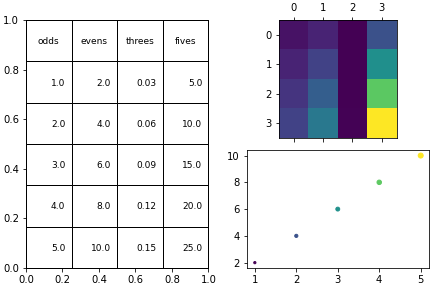
\includegraphics[width=.5\textwidth]{figures/intro/viz_same.png}
    \caption[]{Implicit in visualization is the assumption that these three representations of data are equivalent, specifically that the measurements within a variable and relations of the measurements of each variable are preserved. }
    \label{fig:viz_same}
\end{figure}

\subsection{Thesis statement}
We define a visualization as a transform from data to graphic that preserves the topology of the data and the properties of the measurement type. In fig~\ref{fig:viz_same}, we implicitly assume that the translation from table to heatmap has preserved the order of observations (the rows) and that the perceptually uniform sequential colormap has been applied such that the ordering relation on floats matches the ordering on the colormap (darker colors map to larger numbers). We also make this assumption about color in the scatter map, and that the translation to size and position on screen also respect the ordering on floats. In this work, we propose to mathematically describe the transform of data to visual space such that we can make explicit the implicit topology and types visualizations preserve. We then propose a new architecture for the Python visualization library Matplotlib \cite{hunterMatplotlib2DGraphics2007} based on these descriptions because the Matplolib artist layer is analogous to the transforms. 


\section{Notation \& Definitions}
System of transforms:
input: data w/ structure on fiber bundle + measurement type
artist: data -> visualization
(what structure of input is preserved in output)
we can provide list of
artist : topology it preserves
point/line/face parameters: measurement type properties 

ex: 
Line2D preserves continuity
Linestyle: categorical 

%%define basic properties of measurement of types in a theoretical way or C&P from a paper

Miniumum assumption a transform will make - is this a valid transform for the slot? 

Set of questions/rules to apply such that see a new artist can be defined which lets us maybe simplify optimizations.  

M, Fiber Bundle, Section, operatons on \{data, visual\}, transform data space \& visual space,  

topology gives us that m is preserved
spivak gives us that v is preserved


temperature on globe:
\begin{equation}
data = [[t1], [t2_{la1, lo2}]
fiber = {lat, lon, temp}
m = the data is 2d continous
\end{equation}
artist has implict m
aesthetic paremeters transform in fiber that preserves type operations \& relations in the fiber
lat - relative distance + ordering 

\subsubsection{Graphical Elements}
There is a set of transform functions $T$ that maps from the data space $D$ to the visual space composed of geometric marks and aesthetic channels $V$ \cite{bertinIIPropertiesGraphic2011, munznerMarksChannels}.  We propose that a visualization is 
\begin{equation}
    T: D \rightarrow V
\end{equation}

Wilkenson proposes  that visualization is  \cite{wilkinsonGrammarGraphics2005, wilkinsonMathematicalFoundationAnalytic2010}

\begin{align}
\label{eq:gog_data_range}
G &= {(x, f(x)): x \in R and f(x)=e^{-x^2}}\\
F &= [-3,3] x [0,1]
\end{align}

\begin{equation}
\label{eq:gog_aesthetic_mapping}
A: x \mapsto x_{position}, f(x) \mapsto y_{position}
\end{equation}

\begin{equation}
G_{A} = A(F \cap G) 
\end{equation}

Wilkenson formulates plotting in terms of varsets, which are sets of variables where variables are:
\begin{equation}
V:O\mapsto V    
\end{equation}
Wilkenson's data algebra is equivalent to data reshapes and join and therefore \cite{wickhamLayeredGrammarGraphics2010,wilkinsonGrammarGraphics2005}


\subsection{What is the artist}
Visualization is a two step process where the artists $A$ transforms the data into visual encodings $V$ and then the renderer $R$ transfroms the encodings $V$ to the set of pixels in $P$.
\begin{equation}
    \label{eq:artist}
    A: D \mapsto M
\end{equation}
TYPES: A(D) = M
Spivak A is analogous DT

D is the type  which means it's indexexer K(M/indexer) + V (fiber bundle)
d is a section of a bundle is the data is the values given keys on m + vars on V (c in C)
a(d) = M

$M$ is a composition of the visual channels applied as ....
Is also a CW/simplicial complex/simplacial set 

Channels are ducktyping the variable types
Marks are encoding seperability 

Marks are mapping of simplacial complex into RGB space

(find paper on complex marks)

for every key value in M, have coordinates in the fiber (space)
section: keys -> values 

Scatter Plot:
K - 0D disconnected points
\begin{multline}
A: (C1, C2, C3...)\mapsto (M....)\\
t \in A
\end{multline}

-> preserve type operation and relation

M is the disjoint collection of the output of all these transformers where the transformers preserve the relation and order. 

Line Plot:
L - 1D, can be a function on an interval [a,b]
functions in the column...f(key) -> values

invariance: The symmetry group $A$ preserves invariance when the transforms $a \in A$ are symmetric such that $operation(column) = operation(channel)$ and $operation on data -> operation (mark)$

K might have symmetry -> move back and forth in time, preserved in K
symmatry in fibers -> scaled up/down, categorical,
preserved in the visual variables

groups on K and fibers and subgroups w/ different types and temperatures (Steven's fundemental data types-measurment scales and types)

intervals can transalte, ratio can only scale
group of fibers has to do w/ measurment types
channels themselves independent of data have their own symmatery

(make table of what symmateries are preserved)
visual transformation groups

instead of inputting parameter into input, get to all the other parameters - base thing is a square, 
preserved: operation(D) <-> operation (M)
if A(g*d) = A(d)*g

normalizations of scales in mpl - devision usually leaves same picture but axis is affected - visually length got uniformally smaller but we changed ticks to compensate
Axes has rules about how transform affects it - inside graph invariance is preserved

groups:
symmteries of K
symmetries of cartesian product of columns
each visual channel has symmtery group associated w/
orbit- space of possible visualiztions by changing the constants of each aesthetic (or $f_{red} \rightarrow f_{green}$)  
visual type might be orbit of that (orbit of function in space)->single function that can be transformed in that way
each visualization type is an orbit \& then try to set up equivalence on these...

artist will respect that w/ equivariance, knob on one side will tweak knob on another

Steven's defines the group

Wiki: Symmetry group is the group of all transformations under which the object is invariant. 
The aesthetic transfroms $a \in A$ are a symmetry group that preserves transforms:

\begin{table}
    \label{tab:sym_mark}
    \begin{tabular}{|r|r|}
    \end{tabular}
\caption{Symmetrys one the data preserved with each type of mark\cite{bertinIIPropertiesGraphic2011,munznerMarksChannels}}
\end{table}

\begin{table}
    \label{tab:sym_mark}
    \begin{tabular}{|r|r|}
    \end{tabular}
\caption{Symmetrys one the data preserved with each type of mark\cite{bertinIIPropertiesGraphic2011,munznerMarksChannels}}
\end{table}


Scatter Plot:
K - 0D disconnected points
\begin{multline}
A: (C1, C2, C3...)\mapsto (M....)\\
 t \in A 
\end{multline}

-> preserve type operation and relation

M is the disjoint collection of the output of all these transformers where the transformers preserve the relation and order. M is a bunch of disconnected Marks

Line Plot:
L - 1D, can be a function on an interval [a,b]
functions in the column...f(key) -> values

Box chart: area + scatter 


Combining 
\begin{equation}
    \label{eg:renderer}
    R: M \mapsto P
\end{equation}
Where $P$ is the set of pixels rendered to screen ${p_{i,j} \in P}$


An artist is a function F from X to Y
that satisfyies properties P1, ... PN
Step 1: Define X
step 2: Define Y
Spefiy Pi in terms of equations.


\subsection{visual variables}
Bertin's proposed an organization of visual variables \cite{bertinIIPropertiesGraphic2011} 


\subsection{Grammar of Graphics \& ggplot}
Specifies the end chart (graphic)
we want to specify the transformations ....
\begin{figure}
    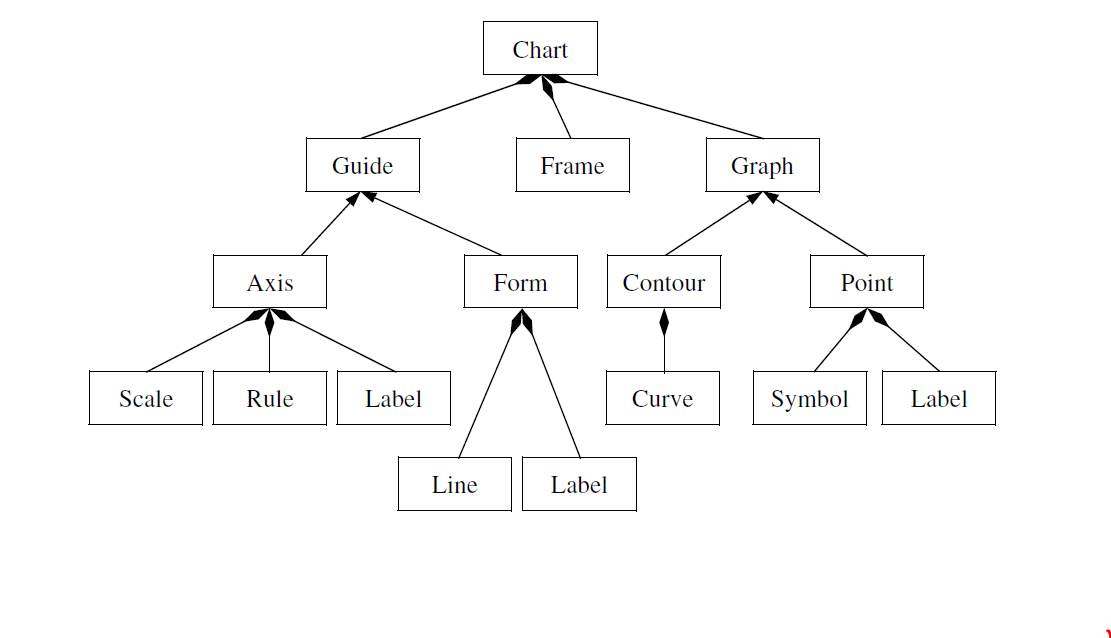
\includegraphics{figures/intro/grammar_chart_composition.png}
    \caption{page 10 (introduction)}
\end{figure}

\begin{figure}
    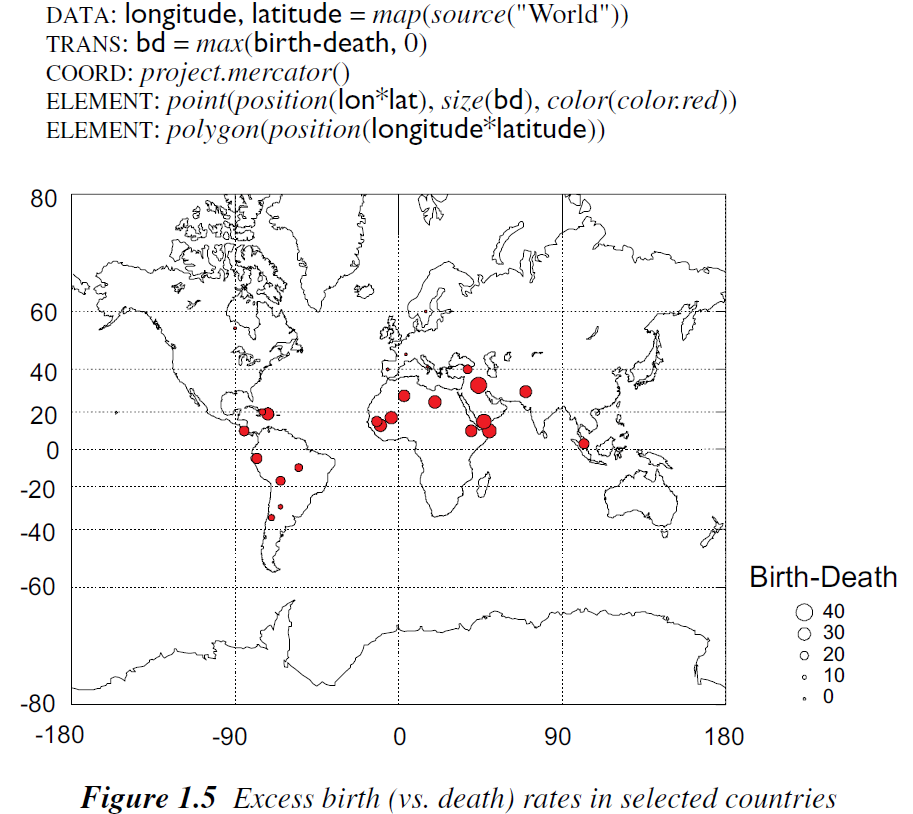
\includegraphics{figures/intro/grammar_example.png}
    \caption{Wilkenson decomposed a graphic into ...} 
\end{figure}

charts - words 
    - instances of much more general objects (geometric primatives)
    - histogram =/= bar chart
graphics - statements 
expliceltly OO
    1. specification
        data - operations/computations
        trans - variable transforms (rank)
        scale - scale transforms
        coord - coordinate system
        element - marks and channels
        guide - meta elements - (axes, legends, etc)
    2. assembly - kinda what happens in artist (spec->something that can go to renderer) 
    3. display - rendering

How is our proposal different? seperation in spec between what's data, aesthetics, and render specific, and what part of the architecture owns those operations


ggplot - strictly hierarchal components (layers), matplotlib - transforms that mostly happen indepently 
"designing and producing statistical graphics is not an art" - ties in w/ difference between drawing program and visualization library, preservation of properties of measurement type and observation type \cite{wickhamGgplot2ElegantGraphics2016}

history of viz - collins, friendly


Wilkenson suggests that the graphics pipeline could be implemented functionally but does not push it in any direction. 

ordering: processed before plotted, 
scales before stats, marks before channels
\begin{figure}
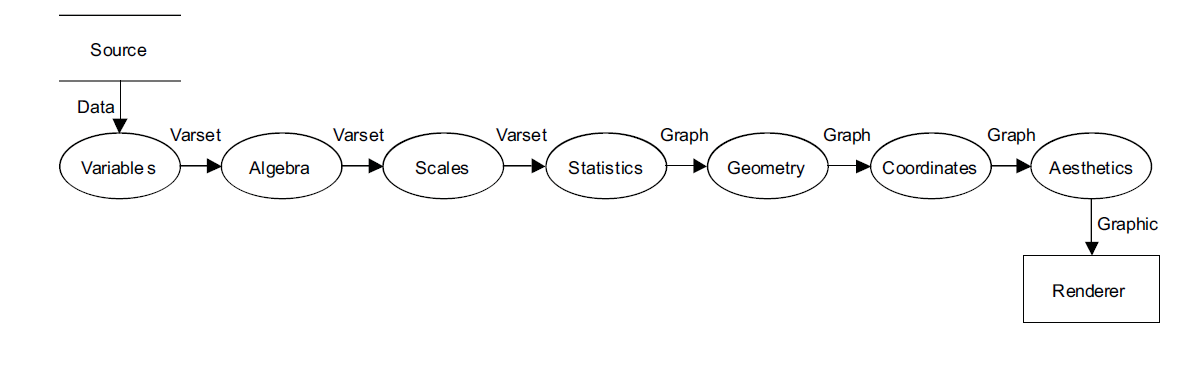
\includegraphics[]{figures/intro/gog_pathway.png}
\caption{Diagram of Grammar of Graphics stages of visualization. Fig 2.2 from chapter 2 of The Grammar of Graphics\cite{wilkinsonGrammarGraphics2005}}
\label{fig:gog_pathway}
\end{figure}
In grammar of graphics, as shown in figure~\ref{fig:gog_pathway} data is extracted from the database one variable at a time with an associated index (primary key). The algebra stage joins the variables to become the varset, which is a flat table where the columns are the variables/attributes, each row is an observation/item, and each cell contains a measurement \cite{munznerChDataAbstraction}. Wilkenson then describes the constraints of the measurement space for each variable through scales \cite{wilkinsonGrammarGraphics2005} with implicit assumptions of the data constraints. After this step, data is transformed computationally in service of the visualization. Some of the variables are then mapped into geometric marks (symbols) and are scaled (height, width) as appropriate. These mappings are then transformed into the coordinate system of the target graph. Then the aesthethic attributes (Bertin's retinal variables, also called channels) such as color or  texture) are applied. Finally

Wilkenson's thoughts on coherancy are equivalent to invariance but less? formally stated \dots

"To call these charts meainingul, defenders must falsify specific assumptions of GoG" \cite{wilkinsonMathematicalFoundationAnalytic2010}


gog implementationss:
\begin{enumerate}
    \item SPSS nViZn
    \item tableu
    \item ggplot
    \item protoviz\d3
    \item vega (interactive GoG)
\end{enumerate}


\printbibliography
\end{document}